% !Mode:: "TeX:UTF-8"

\chapter{绪论}[Introduction]

\section{课题背景及研究的目的和意义}[Background]
知识图谱作为人工智能的重要基石,近些年得到了不断的发展和应用。特别是搜索引擎开始利用知识图谱来改进搜索的质量,加快搜索的速度,并且实现语义搜索和推理。

知识图谱是由语义表示的网络,它能够帮助使用者搜索知识网络中的所有知识。知识网络是由许多个实体,属性和属性值构成的。有全局唯一的标识符URI来表示一个实体,属性是用来描述实体的内在特性或实体之间的关联关系。W3C提出了一种资源描述框架RDF\cite{rdf}来表示知识图谱网络,一条知识表示为一个SPO三元组(Subject,Predicate,Object)。如果从图的角度来看RDF数据的话,RDF的实体或属性值是图的顶点,RDF的属性是图的边。为了方便RDF数据的检索,W3C组织还提出了一种类似于SQL的形式化查询语言SPARQL\cite{sparql}。SPARQL查询的基本单位是三元组模式(triple pattern),多个三元组模式通过多种运算符形成更多复杂的图模式。SPARQL查询是将查询问题转化为图上的子图匹配问题,因为这一过程可以看作在RDF图中找到全部满足查询图模式的匹配。

随着知识图谱应用的广泛使用,到目前为止,规模为百万顶点(106)和上亿条边(108)的知识图谱数据集已经比较常见\cite{MassiveData},根据链接开放数据2018年8月发布的LOD云图中很多知识图谱数据集规模超过10亿条三元组。例如,维基百科知识图谱DBpedia(>30亿条)、地理信息知识图谱LinkedGeoData(>30亿条)和蛋白质知识图谱UniProt(>130亿条)等。在数据量如此巨大的情况下,实际应用场景对图数据库的查询性能提出了更高的要求。在此情况下,对图数据库性能的优化,尤其是对SPARQL的查询优化显得尤为重要。

近年来人工智能的迅速发展为数据库查询问题提供了新的机会\cite{MLforDB}。人工智能技术强大的适应性和数据表征能力能够智能地对大量、复杂、动态的数据和工作负载进行深入的分析。在现有工作中,已有许多基于机器学习的数据管理技术被提出。研究人员分别从数据库系统调优和查询优化两方面出发,提出了如SageDB\cite{SageDB}、GALO\cite{GALO}、Neo\cite{Neo}、
SkinnerDB\cite{SkinnerDB}等人工智能赋能的数据库新技术。

虽然研究人员利用人工智能技术针对查询优化已经进行了很多研究工作,但是它们大多是面向关系数据库的,而尚未有研究关注针对图数据库的智能查询优化问题。因此,基于人工智能的图数据查询优化问题亟待解决。

综上所述,由于图数据库中的RDF数据规模不断增大,需要优化SPARQL查询过程才能继续满足应用对查询的效率要求。研究人员应用人工智能技术在SQL的查询优化中已经取得了显著的成效,而且尚未有人应用人工智能针对SPARQL进行优化,所以本课题使用人工智能技术对SPARQL查询进行优化是有价值有必要的。


\section{国内外研究现状}[Research status]

\subsection{人工智能在关系数据库查询的优化}[Research status in SQL]
查询优化问题已经被研究了四十多年,至今仍然是一个活跃的研究领域。该问题的组合复杂性使得启发式算法得以普遍应用[7-9]。许多商用DBMS的查询优化策略都是基于System R [2]或Volcano Optimizer Generator [8]中引入的思想。这些系统使用了动态规划(DP)并结合一组规则来找到好的查询计划。这些规则缩减了潜在查询计划的搜索空间,减少了优化查询所花费的时间,但也会降低在大型搜索空间中找到最佳查询计划的可能性。传统查询优化方法除了搜索策略的局限性外,还存在第二个问题:它们依靠代价模型来估计执行查询的成本。这些代价模型建立在基数估计的基础上,基数估计大多基于分位数统计,频率分析或没有理论基础的方法[16]。基数估计中的错误通常会导致查询计划的效率不够理想。此外,传统的查询优化器无法从先前执行的查询中学习。

受机器学习最新进展的启发,数据库研究的一个新趋势是将启发式算法用学习方法代替。因此,Krishnan等人探索了使用学习方法合成特定数据集的连接搜索策略[10]。假设一个给定的代价模型和计划空间,研究是否能够对一个特定数据集上所有可能的连接计划进行搜索。这一问题的目标是从之前能够大幅度减少搜索时间的计划中学习到适合的搜索策略。Krishnan等人的主要发现是连接排序与强化学习有深层次的算法联系,即连接排序的顺序结构也是支持强化学习问题的结构。所以,Krishnan等人利用这一算法上的联系将强化学习嵌入到传统的查询优化器中,建立了一个基于强化学习的优化器DQ。该优化器优化了选择-投影-连接、查询连接以及物理操作符选择,能够根据之前执行查询计划的结果训练一个强化学习模型,从而有效完善后续的查询操作。

Marcus等人也将深度强化学习应用于查询优化中,提出了一个自动查询优化器,使得优化器。此外,该优化器紧密结合能够自动调整特定的数据库,无需专业数据库管理员的干预[11]过去查询优化和执行的经验反馈,从而显著提高了查询性能。Marcus等人还提出了一个依赖深度神经网络来生成查询执行计划的查询优化器Neo[5]。该优化器从已有的优化器生成查询优化模型,并持续根据到来的查询学习,从成功的查询中建立模型,从失败的查询中进一步学习调整。此外,Neo优化器能够适应不同的数据模式,且能够容忍一定的估计错误。

\subsection{SPARQL查询优化的研究}[Research status in SPARQL]在SPARQL查询优化的方向上,也有很多研究者做出了努力。Markus在ARQ(ApacheSPARQLProcessor)的基础上进行了改进[12],做出了optARQ原型,它通过建立选择性估计索引的方式,来最小化查询中间结果的生成数量,从而提高查询的效率。Groppe认为SPARQL语言不够精简[13],他提出了SPARQL语言的核心部分,并称之为coreSPARQL,它具有与SPARQL相同的表达能力,但是消除了SPARQL的冗余语言构造,而且它的语法对机器更加友好。Groppe将SPARQL语言转换为coreSPARQL语言,并开发了一组重写规则来优化coreSPRQL查询,以此来提高执行效率。

国内学者在SPARQL的查询优化上也做出了很多的努力。武汉大学信息资源研究中心提出了一种优化方法[14],他们使用RDF模式信息来精简SPARQL基本图模式,然后使用B树结构快速估计SPARQL连接图的节点大小及边权值,使用连接代价估计并结合动态规划方法找到最优逻辑查询计划。除了这种基于传统算法的优化方法,启发式算法也得到了大量的应用,例如,有学者提出了一种基于精英蚁群算法与权重矩阵的SPARQL查询优化算法[15],他针对不同的图形状设计了有效的权重矩阵模型,为不同的查询形状设置了专门的优化参数,然后将权重矩阵作为蚁群算法的输入参数,分别利用人工蚁群与精英蚁群方法对SPARQL不同形状的查询语句进行优化。

\subsection{研究现状分析}[Research status analytics]
根据国内外对SPARQL查询优化的研究内容,对研究现状的分析如下:

(1)应用人工智能技术在SQL的查询优化中已经取得了显著的成效,例如Neo查询优化器和DQ查询优化器,其性能较传统方法有极大的提升而且还能在查询流中进行自学习,不断提升适应能力和查询
效率。

(2)现有的针对SPARQL的查询优化主要是改进代价估计模型,精简SPARQL语言和改进RDF的存储方式,这些方法与SQL查询优化的研究一样,都存在搜索空间不足和代价估计模型不够准确的问题,而
采用人工智能技术的研究还没有。


\section{本文研究内容和结构安排}[Research content and structure]
本文的主要研究内容为基于人工智能的SPARQL的查询优化技术,采用了强化学习对SPARQL中的连接顺序进行优化,文章的主要章节如下:

第一章为绪论部分,开始介绍了本课题的研究背景和本研究的目的意义,然后对目前国内外对SPARQL查询优化的现状进行了分析和总结,最后给出了本文的研究内容和结构安排。

第二章介绍了本文用到的查询优化的基础知识。首先我们介绍了RDF图模型和本文的主要研究对象SPARQL查询语言,并给出了其相关概念的形式化定义和示例。然后我们又详细描述了强化学习的概念和本文将要用到的算法。最后我们介绍了图数据库中最常用的Jena框架。

第三章介绍了基于强化学习的SPARQL查询优化的方法。我们首先详细得描述了SPARQL的基本图模式优化问题并确定了该优化问题的输出输出。之后,我们从马尔可夫决策过程的五元组(状态,动作,策略,奖励,初始状态)开始,分别详细得介绍了状态、初始状态、动作的定义和特征化方法,然后通过举例的方式描述了状态之间的转换方式,最后介绍了奖励值的计算方法。

第四章介绍了强化学习算法的实现,包括Q学习算法和深度Q学习算法的实现和改进。之后介绍了实验的环境,包括CPU、GPU、操作系统和基准测试。最后,给出了实验中两种算法的实测结果,通过与随机连接顺序的查询效率和Jena自带优化器查询效率进行比较,来验证本文优化方法的有效性。

\chapter{预备知识}[Preliminary knowledge]

\section{RDF图模型}

RDF全称为资源描述框架(resource description framework),是万维网联盟(World Wide Web consortium,简称W3C)制定的在语义Web(semantic Web)上表示和交换机器可理解
(machine-understandable)信息的标准数据模型[23]。在互联网中,所有能够用RDF数据表示的对象都称之为资源,例如所有的事物、概念和信息等。资源通常情况下使用唯一资源标识符(URI)来表示。在RDF图中,每个资源具有一个HTTP URI作为其唯一id。

 \begin{definition}[RDF项(RDF Term)]    
    用I来表示IRI的集合
    用RDF-L来表示文本信息(Literals)的集合
    用RDF-B来表示空值(Blank nodes)的集合
    用RDF-T来表示RDF项(RDF Term)
\end{definition}

\begin{definition}[(RDF三元组)]    
    RDF三元组是形如(s,p,o)的数据组合,又被称为声明。其中s代表主体(subject),p代表属性(property),
    o代表客体(object)。三元组的选取区间可以表示为$(I\bigcup RDF-B)\times(I\bigcup RDF-B)\times(I\bigcup RDF-B\bigcup RDF-L)$。
    
    例如,对于三元组<Tony, graduateFrom, HIT>,Tony代表主体,graduateFrom(毕业于)代表属性,HIT代表客体。三元组的意思是Tony毕业于HIT。
\end{definition}

\begin{table}[htbp]
    \caption[table1]{RDF数据}
    \label{RDF1}
    \vspace{0.5em}\centering\wuhao
    \begin{tabular}{|c|}
    \toprule[1.5pt]
    RDF三元组\\
    \midrule[1pt]    
    <student1,rdf:type,Student>\\
    <student1,telephone,"xxx-xxxx-xxxx">\\
    <student1,takesCourse,course1>\\
    <student1,memberOf,department>\\
    <student1,advisor,teacher2>\\
    <course1,rdf:type,Course>\\
    <teacher2,teacherOf,course1>\\
    <teacher2,teacherOf,course3>\\
    <teacher2,worksFor,department1>\\
    <department1,subOrganizationOf,university0>\\
    <student4,takeCourse,course1>\\
    <student4,takeCourse,course4>\\
    <student4,email."xx@edu.com">\\
    <teacher1,teacherOf,course4>\\
    \bottomrule[1.5pt]
    \end{tabular}
\end{table}

\begin{figure}[h]
    \centering
    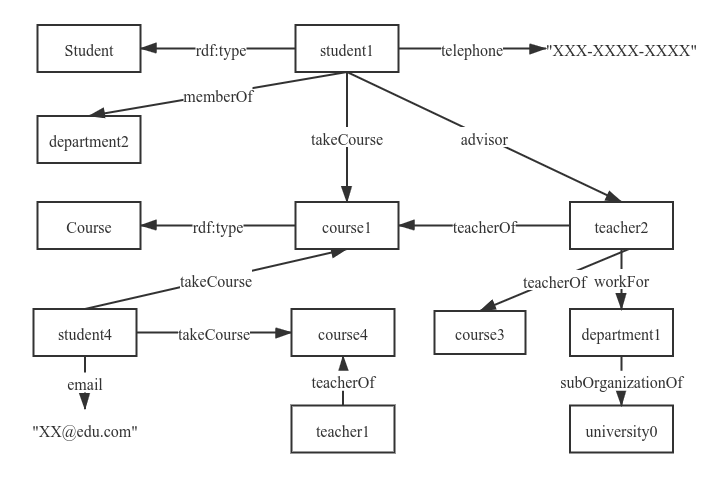
\includegraphics[width = 1\textwidth]{RDF}
    \caption{RDF图模型}
    \label{RDFPhoto}
\end{figure}

表格\ref{RDF1}是一个包含14个RDF三元组的数据集,图\ref{RDFPhoto}是表格\ref{RDF1}RDF数据对应的图模型表示,其中方框表示实体,双引号中的数值表示属性值,图上的边表示属性值。


\section{SPARQL语言与查询过程}

SPARQL(simple protocol and RDF query language)是W3C提出的用于检索RDF数据的形式化查询语言,也是目前使用最广泛的查询语言。类似于SQL,SPARQL支持多种查询格式,例如SELECT、ASK、DESCRIBE、CONSTRUCT。其中,SELECT查询格式用于标准查询,以标准的 SPARQL XML 结果格式返回查询结果。ASK 查询返回结果是 yes 或 no,没有具体内容。DESCRIBE 用于提取本体和实例数据的一部分,返回一个图形,其中包含和图形模式匹配的节点的相关信息。
\begin{definition}[(三元组模式)] 
    \label{Triple}   
    一个三元组模式(Triple Pattern)是集合$(RDF-T \bigcup V)\times(I \bigcup V)\times(RDF-T \bigcup V)$的一项,其中V代表变量。三元组模式常用$(s,p,o)$来表示。
\end{definition}
\begin{definition}[基本图模式(BGP)]    
    \label{BGP}
    一个基本图模式是$$\wedge_{1\leqslant i\leqslant m}(s_i,p_i,o_i)$$
    其中
    \begin{enumerate}
        \item $(s_i,p_i,o_i)$是一个三元组模式$(1 \leqslant  i \leqslant m)$。
        \item $\wedge$表示逻辑合取。
    \end{enumerate}
    
\end{definition}
图...是一个示例SPARQL查询,其中WHERE子句是查询的主要组成部分,包含6个基本的三元组模式(triple pattern),其中三元组模式通过对RDF三元组中的主体,属性或客体进行变量替换得到。

SPARQL查询过程 中,用户(包括人和机器)通过一系列接口与系统进行交互,接口将查询请求送入SPARQL查询处理器,调用底层的RDF存储获取相关的结果记录。SPARQL通过查询器扫描关键词,并且根据
标准解析查询序列验证RDF三元组的有效性。如果查询不正确,则在处理的过程中及时通过接口为用户返回错误信息,如图\ref{SPARQL查询过程}所示:

在 SPARQL 处理器中,首先利用解析器对查询语句进行解析,判断是否存在语法错误。接着在重写查询阶段,以规则为基础重新优化查询语句。最后通过执行查询计划发生器产生的计划获取RDF数据并通过接口返回给用户。
\begin{figure}[h]
\centering
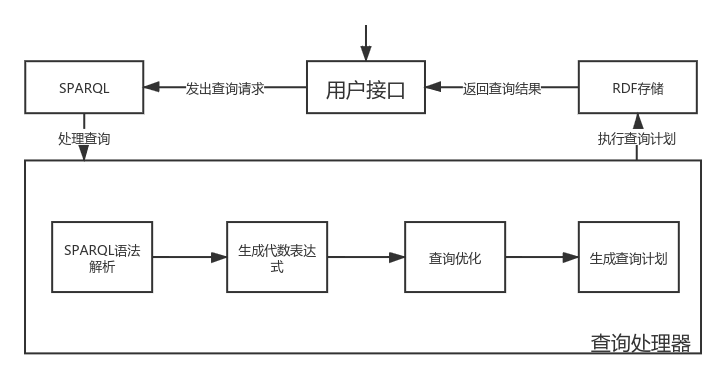
\includegraphics[width = 1\textwidth]{SPARQL}
\caption{SPARQL查询过程}
\label{SPARQL查询过程}
\end{figure}

\section{强化学习}[Reinforcement Learning]
\subsection{概述}[introduction]
强化学习(Reinforcement learning)\cite{RLIntroduction}是机器学习中的一个领域,这种方法主要思想是通过与环境的交互来学习。其来源于心理学中的行为主义理论,即有机体如何在环境给予的奖励或惩罚的刺激下,逐步形成对刺激的预期,产生能获得最大利益的习惯性行为。例如当婴儿开始学习走路时,他刚开始并不能掌握平衡,并不会直接学会走路,但他通过与周围环境的交互获得反馈,例如摔倒会给他带来疼痛感(惩罚),顺利走出第一步保持了平衡(奖励),婴儿就会知道每个动作的后果(获得惩罚或奖励),从而逐渐选择奖励最多的动作,直到完全学会走路(奖励最大化)。当我们从计算机科学的角度看待这种方法时,我们可以将其解释为一个函数。该函数尝试使奖励信号最大化,而无需告知必须采取何种行动。

很多形式的有监督机器学习方法通常都有很多的输入输出对,每一个输入输出都是提前备好的训练数据集,训练过程会被告知要采取哪些动作,但是强化学习不同于前者的是它必须通过尝试不同的动作,根据与环境的交互获得动作的反馈,从而确定采取哪些动作能产生最大的回报。强化学习更加专注于在线规划,需要在探索(在未知的领域)和遵从(现有知识)之间找到平衡。

\subsection{马尔可夫决策过程}[MDP]
从技术角度来看,强化学习是一种随机优化方法,它可以表述为马尔可夫决策过程(MDP)\cite{MDP}。其基本思想是,代理(agent)采取一系列行动,以优化MDP模型中的给定目标。马尔可夫决策过程(MDP)是马尔可夫链(Markov Chains)的拓展,所以它需要满足马尔可夫链的属性。例如未来状态的进展仅取决于当前状态,而不取决于过去的状态和采取的动作。一个马尔可夫决策过程可以形式化的表示为以下五元组:
\begin{equation}\label{MDP5}
\langle S, A, P(s,a),R(s,a),S_0 \rangle
\end{equation}
\begin{itemize}
    \item S代表Agent所有可能的状态。
    \item A代表Agent可以采取的所有动作来到达一下个状态。
    \item $S_{t+1}\sim P(s,a)$是在状态s通过采取动作a到达的新状态。
    \item $R(s,a)$代表在状态s通过采取动作a获得的奖励。
    \item $S_0$是在Agent初始时的状态。
\end{itemize}

总体的目标是找到一个决策策略$\pi :S\longmapsto A$(一个状态到动作的映射函数),使得期望的奖励最大化。马尔可夫决策过程是一个从交互中学习的过程,\ref{Interaction}表示出了这个交互学习过程:Agent是学习者,它在某个状态下采取动作并且与环境交互,Agent从环境中获取到下一个状态和动作对应的奖励。状态信息通常需要编码,也被称为observations。
\begin{figure}[h]
    \centering
    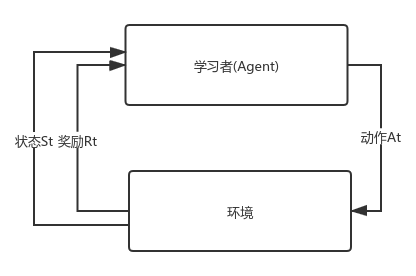
\includegraphics[width = 1\textwidth]{MDP}
    \caption{马尔可夫决策学习者与环境交互过程}
    \label{Interaction}
\end{figure}

\subsection{Q学习算法}
Q学习算法\cite{QLearning2}是由Watkins在其博士论文"Learning from delayed rewards"\cite{QLearning0}中第一次提出的,该算法是强化学习中具有里程碑意义的算法。Q学习算法是时间差分算法(TD)\cite{QLearning1}的一种,也是一种模型无关的算法,其主要针对具有折扣的奖励指标的控制。
Q学习算法\cite{QLearning2}是由Watkins在其博士论文"Learning from delayed rewards"\cite{QLearning0}中第一次提出的,该算法是强化学习中具有里程碑意义的算法。Q学习算法是时间差分算法(TD)\cite{QLearning1}的一种,也是一种模型无关的算法,其主要针对具有折扣的奖励指标的控制。

Q学习算法在迭代时针对状态-动作对进行奖惩,Q(s,a)作为在状态s下执行动作a后获得的累计回报,即Q值函数。Q值函数取决于当前的立即回报和期望的延时回报,因此,学习系统每一次学习迭代都需要考察当前的这个动作。Q学习算法的最佳策略为当前状态s下累计回报值最大时对应的策略,即:
\begin{equation}
    \pi^*(s) = max Q(s,a)
\end{equation}

Q值表是所有状态-动作对与其对应的Q值组成的一张二维表,每次迭代,这张表的值就更新一次。在学习的过程中,通过不断更新Q值表中状态-动作对所对应的Q值,从而对Q值表进行更新。随着学习次数的增加,Q值表逐渐趋于稳定,即收敛。学习系统在之后做决策的时候,根据Q学习算法学习到的Q值表(经验)做出决策,同时,针对新变化的状态留有一定的学习余地,使得Q学习算法更适用于动态变化的环境。

在t时刻,当前环境的状态为$s_t$,学习者选择了动作$a_i$,并且执行这个动作,经过与环境的交互,学习者的状态由$s_t$变成了$s_{t+1}$,并且环境反馈给学习者一个反馈值$r$,算法根据公式\ref{QValue}\cite{RLIntroduction}更新Q值表:
\begin{equation}
    \label{QValue}
    Q(s_t,a_i)=(1-\alpha)*Q(s_t,a_i)+\alpha *[r(s_t,a_i)+\gamma *maxQ(s_{t+1},a)]
\end{equation}

其中

$\alpha$是学习因子,$0<\alpha <1$;

$\gamma$是折扣因子,$0<\gamma <1$;

$r(s_t,\alpha_i)$:在t时刻学习者在状态$s_t$,执行动作$\alpha_i$从环境获得的回报;

$Q(s_t,\alpha_i)$:策略$\pi=(s_t,\alpha_i)$所对应的累计奖赏值;

在动作选择的过程中,需要用到动作选择策略,可以使用随机动作法,也常采用贪心策略($\varepsilon-greedy$),即学习者在选择动作时,以$\varepsilon$的概率自由探索,以$1-\varepsilon$的概率根据学习的经验选择动作。动作选择策略只需要满足一定条件就能保证Q函数最终收敛,Watkins在论文\cite{QLearning3}中证明了学习算法的收敛性。所以,Q学习算法是一种非常有效的模型无关的强化学习算法。

Q学习算法的执行步骤如下:
\begin{enumerate}
    \item 初始化。初始化学习因子、折扣因子和Q值表,t=0;
    \item 初始化当前的状态$s_t$;
    \item 根据当前状态$s_t$,Q学习算法选择一个动作$a_i$;
    \item 执行动作$a_i$,并确定下一个时刻的新状态$s_{t+1}$和环境的奖励$r$;
    \item 根据公式\ref{QValue}更新Q值表,设置$t = t+1$;
    \item 判断是否满足终止状态的条件,若满足,则结束算法,否则,返回到第二步。
\end{enumerate}

\subsection{深度Q学习算法(DQN)}[DQN]
Q学习算法能够较好地解决很多问题,但是如果在情况较为复杂,状态与动作的组合太多甚至无限多的时候,Q矩阵的存储容量和计算复杂度将会急剧上升。为了解决这个问题,Graves等人提出了结合深度学习与Q学习的算法深度Q学习网络算法\cite{DQNNature},也被广泛地称为DQN。目前,DQN受到了许多关注和探索,不仅被应用于自动控制领域,也被尝试应用于包括计算机视觉领域在内的其他领域。

一般而言,深度学习与强化学习结合的思路有以下几种:利用深度神经网络来模拟环境,即输出动作对状态的改变方式和相应的回报值;利用深度神经网络来估计Q值函数;直接利用深度神经网络来学习策略。DQN属于第二种,可以通过神经网络回归拟合出Q值的近似值,而不是像Q学习算法一样记住所有的Q值。

强化学习结合深度学习的困难指出在于:
\begin{enumerate}    
    \item 深度学习的成功依赖于大量的标注样本,从而能够进行有监督学习,而强化学习只有一个奖励值$r$,而且这个值总是伴随有噪声、延迟和稀疏性,无法给每一个状态一个即时的回报作为监督信息。
    \item 深度学习的样本都是独立的,而强化学习中的状态与状态之间是具有相关性的,前后的状态之间会相互影响。
    \item 深度学习的目标分布是固定的,例如图像分类任务中,猫就是猫,不会随时间改变。然而强化学习中的输入和学习目标都在随着决策的过程不断改变,使得训练十分不稳定。
\end{enumerate}

为了解决这些困难,DQN提出了两个关键的技术:经验回放(Experience replay)和目标网络(Target network),使用Q学习来为神经网络提供有监督数据,保证了DQN的训练与普通的监督学习保持一致。

经验回放就是建立一个经验池,把每次训练收集到的经验都保存起来,这里的经验是指学习者状态间的转移和相应的回报,在训练的时候,随机从这个经验池中采样一个批次的数据作为深度神经网络的训练数据。由于从经验池中采样数据的操作是随机的,所以采样所得的训练数据可以近似认为是独立同分布的,这样就可以满足深度神经网络对训练数据的要求。其中,动作的选择一般采用常规的贪心策略($\varepsilon-greedy$)。

目标网络是一种训练技巧,其通过构造两个一模一样的网络$\theta$和$\theta^{'}$,利用$\theta$来进行Q值的回归但是不对其参数进行更新,$\theta^{'}$网络的参数则随着训练的过程不断更新,在训练达到一定的迭代次数后,再将$\theta^{'}$中的参数赋值给$\theta$中。这样做的目的是在一定时间内保证目标(Q值)网络的稳定,避免了网络训练过程中去拟合一个随时变化的目标分布。此外,由于网络训练的过程中,目标网络参数$\theta$的参数不是即时变化的,所以尽管训练的数据不是完全独立同分布的,对网络训练的影响也会减小。

DQN算法见伪代码\ref{DQN伪代码}:
\begin{algorithm}
    \caption{DQN算法}
    \label{DQN伪代码}    
    初始化容量为N的经验池D\;
    以随机参数初始化动作值函数Q\;
    \For{episode = 1 to $M$}  
    {
        初始化状态序列$s_1$ = {$x_1$},预处理后的状态序列$\phi_1 = \phi(s_1) $\;
        \For{$t$=1 to $T$}
        {
            以概率$\varepsilon$选择一个随机动作$a_t$\;
            否则,$a_t = maxQ^*(\phi(s_t),a;\theta)$\;
            执行$a_t$并求得相应的回报$r_t$和得到新的输入$x_{t+1}$\;
            更新状态$s_{t+1}=s_t$与$\phi_{t+1} = \phi(s_{t+1})$\;
            将$(\phi_i,a_t,r_t,\phi_{t+1})$存进经验池D中\;
            从D中随机采样一个批次的样本$(\phi_i,a_t,r_t,\phi_{t+1})$\;
            求得
            \[
                y_j = \begin{cases}
                    r_j,& \text{for terminal }\phi_{j+1}\\
                    r_j+\gamma max_{\alpha^{'}}Q(\phi_{j+1},a^{'};\theta), & \text{for else } \phi_{j+1}.
                \end{cases};
            \]\\
            利用该监督信息对深度神经网络进行监督学习\;
        }            
    }
\end{algorithm} 

\section{Jena框架简介}
Apache Jena(简写为Jena)是一个免费的开源Java框架,是一个用于构建语义网络和链接数据的应用程序。Jena最初是英国布里斯托尔的HP Labs的研究人员在2000年开发的,并且在2010年称为apache软件基金会的开源项目。Jena一直是一个开源项目,并且已广泛用于各种语义网络应用程序中。

Jena框架由多个不同的API组成,它们相互交互来处理RDF数据。
\begin{figure}[h]
    \centering
    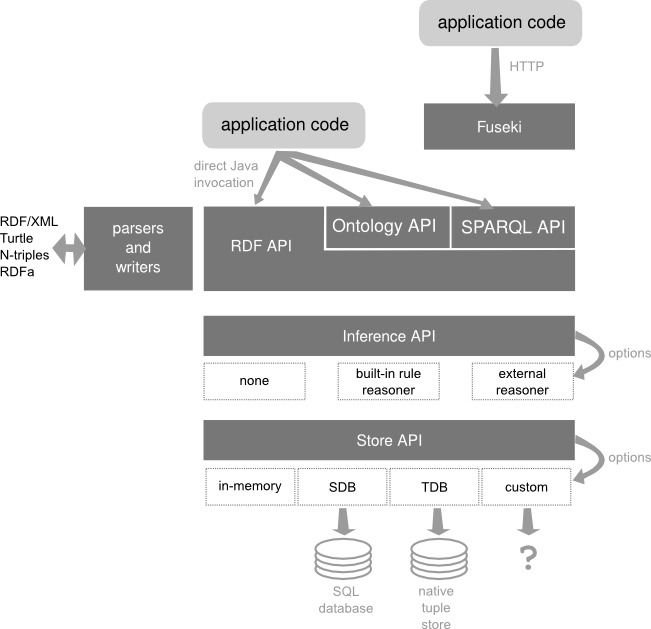
\includegraphics[width = 1\textwidth]{Jena}
    \caption{jena框架}
    \label{Jena}
\end{figure}
其架构结构如图\ref{Jena}所示。

Jena具体的接口和功能主要有:
\begin{enumerate}
    \item RDF模块。RDF单元的主要功能是它可以将RDF信息映射到Java模型中,能够读写和处理RDF数据,同时给其他的模块提供接口。
    \item 查询模块。Jena提供了ARQ查询引擎来负责SPARQL语言的查询功能,实现复杂的知识查询功能。
    \item 本体(Ontology)模块。Ontology模块是基于RDF单元构建的,其最主要的功能是进行OWL相关的操作。Ontology模块中大量的API接口都运用了RDF模块中的技术,可以实现的功能与RDF模块相近。
    \item 基于规则的推理引擎。这个模块提供对本体的类、属性和实例的推理功能,推理器可以由Jena提供,也可以使用外部的推理器。用户可以自己定制推理规则,检测RDF和OWL本体模型的一致性。
    \item 存储模块。这个模块负责持久化存储Model。Jena提供了三种存储方式:
    \begin{enumerate}
        \item 内存模式。该方式是把Model中的信息读取并存储到内存中,因此它的存储速度比其他的存储模式更快,但是这样会受制于本机的内存容量,不适合存储较大规模的模型。
        \item TDB方式。TDB方式是以本地三元组的方式进行存储,是Triple Database的意思。TDB是一个只负责查询与存储OWL/RDF数据的图数据库,而且能够通过SPARQL语言来完成基于图的精确有效的查询。TDB使用的是硬盘的存储方式,拥有较大的存储容量,能够满足大部分用户的存储需求。目前,Jena最推荐且常用的一种存储方式就是TDB。
        \item SDB方式。SDB是一种基于SQL数据库的存储方式。该方式是先分割本体模型中的数据关系,然后把关系保存到关系型数据库中,这种方式可以将Jena框架与已经成熟的SQL数据库连接,使得开发者构建应用时可以利用存有的关系型数据。但是SQL的性能和稳定性都不如TDB的方式。
    \end{enumerate}
    \item 服务机制。Jena提供了Fuseki,它是一个SPARQL服务器。它可以作为操作系统,Java Web应用程序和独立服务器运行。它提供了安全性方面的保障机制(Apache Shiro),并具有用于服务器监视和管理的用户界面。
\end{enumerate}

\section{本章小结}[summary]
在这一章中,我们主要对本文中使用到的基础技术进行了详细的介绍。我们首先介绍了RDF图模型的定义,包括几个重要名词解释和形式化的定义,还介绍了SPARQL查询语言的定义、语法、查询的构成和查询的执行过程,这两个都是本文后续研究的重要对象。之后,又介绍了强化学习的基本概念,马尔可夫决策过程及本文后续要用到的Q学习算法和深度Q学习网络算法。最后,我们还介绍了图数据库中最常用的Jena框架,包括其模块架构和功能。在下一章中,我们将介绍如何使用强化学习来对SPARQL查询过程进行优化。

\chapter{基于强化学习的SPARQL查询优化算法}[RL based SPARQL Optimizer]
在本章中,我们将从马尔可夫决策模型的定义开始,介绍如何定义状态,动作,奖励等要素以及其编码方式,然后详细描述两种强化学习算法的具体实现。

\section{优化问题描述}[BGP]
SPARQL的查询多种多样,其中包括图模式匹配查询,导航式查询和分析性查询这三个大类型,但是最常见最常用的查询是图模式匹配查询。在图模式匹配查询中,基本图模式匹配查询(BGP)又是核心。在如下SPARQL查询语句\ref{sparql1}中:
\begin{lstlisting}[caption={SPARQL查询语句},label={sparql1}]
    PREFIX rdf: <http://www.w3.org/1999/02/22-rdf-syntax-ns#>
    PREFIX ub: <http://www.lehigh.edu/~zhp2/2004/0401/univ-bench.owl#>
    SELECT ?X ?Y ?Z
    WHERE
    {
        ?X rdf:type ub:GraduateStudent .  ------T1
        ?X ub:memberOf ?Z .               ------T2
        ?Z rdf:type ub:Department .       ------T3
        ?Z ub:subOrganizationOf ?Y .      ------T4
        ?Y rdf:type ub:University .       ------T5        
        ?X ub:undergraduateDegreeFrom ?Y  ------T6
    }
\end{lstlisting}
根据定义\ref{Triple},$T_1$到$T_6$是6个三元组模式,根据定义\ref{BGP},$T_1\wedge T_2\wedge T_3\wedge T_4\wedge T_5\wedge T_6$是一个基本图模式(BGP)。

对三元组模式$T_1$的查询结果是如下表\ref{T1}的中间结果:
\begin{table}[htbp]
    \caption[table1]{三元组模式$T_1$的查询中间结果}
    \label{T1}
    \vspace{0.5em}\centering\wuhao
    \begin{tabular}{|c|c|c|}
    \toprule[1.5pt]
    $?X$ & rdf:type & ub:GraduateStudent\\
    \midrule[1pt]
    Department14.University2.GraduateStudent101 & rdf:type & ub:GraduateStudent\\
    Department8.University2.GraduateStudent61 & rdf:type &ub:GraduateStudent\\
    \bottomrule[1.5pt]
    \end{tabular}
\end{table}
三元组模式$T_1$的语义是查询类型是研究生(graduate student)的全部实体。在中间结果表格中,变量$?X$表示的结果是复合条件的全部学生实体的URI。

对三元组模式$T_2$的查询结果是如下表\ref{T2}的中间结果,
\begin{table}[htbp]
    \caption[table1]{三元组模式$T_2$的查询中间结果}
    \label{T2}
    \vspace{0.5em}\centering\wuhao
    \begin{tabular}{|c|c|c|}
    \toprule[1.5pt]
    $?X$ & ub:memberOf & $?Z$\\
    \midrule[1pt]
    Department15.University2.UndergraduateStudent242 & ub:memberOf &Department15.University2\\
    Department14.University2.GraduateStudent101 & ub:memberOf & Department14.University2\\
    Department8.University2.GraduateStudent61 & ub:memberOf &Department8.University2\\    
    \bottomrule[1.5pt]
    \end{tabular}
\end{table}
三元组模式$T_2$的语义是查询$?X$是$?Z$的成员的模式。在中间结果表格中,变量$?X$表示的结果是符合条件的全部学生实体的URI,变量$?Z$表示的结果是所有组织实体的URI,可以看到与表格\ref{T1}中表格中$?X$全是研究生(graduate student)结果不同的是,表格\ref{T2}的第一行出现了本科生(undergraduate student \#242)。

在图数据库处理该SPARQL查询时,会先查询得到三元组模式$T_1$的中间结果\ref{T1},然后再查询得到三元组模式$T_2$的中间结果\ref{T2},之后会将两个中间结果进行连接操作,从而得到新的中间结果如下表\ref{MidResult}所示:
\begin{table}[htbp]
    \caption[table1]{三元组模式$T_1$与$T_2$连接操作后的中间结果}
    \label{MidResult}
    \vspace{0.5em}\centering\wuhao
    \begin{tabular}{|c|c|c|}
    \toprule[1.5pt]
    $?X$ & ub:memberOf & $?Z$\\
    \midrule[1pt]
    Department14.University2.GraduateStudent101 & ub:memberOf & Department14.University2\\
    Department8.University2.GraduateStudent61 & ub:memberOf &Department8.University2\\
    \bottomrule[1.5pt]
    \end{tabular}
\end{table}

从$T_1 \Join T_2 $以此类推,当最后完成$T_1 \Join T_2 \Join T_3 \Join T_4 \Join T_5 \Join T_6$后,将得到SPARQL查询\ref{sparql1}的最终结果。

这6个三元组模式的连接顺序将会对中间结果的大小以及查询所需时间产生巨大的影响。例如,在相同实验环境和相同的数据集规模下,使用连接顺序1:$T_1 \Join T_3 \Join T_2 \Join T_5 \Join T_4 \Join T_6$所需的查询时间实测为6.64s,而使用连接顺序2:$T_3 \Join T_2 \Join T_6 \Join T_4 \Join T_5 \Join T_1$所需的查询时间实测为0.67s,查询时间对比图如图\ref{SequenceTime}所示。由此可见,在基本图模式(BGP)中的三元组模式的连接顺序具有非常大的优化空间,好的连接顺序将比差的连接顺序效率提升9倍左右。同时,连接顺序的空间复杂度是$(n)!$,n是查询中三元组模式的个数,所以较大的解空间也将给查询优化带来很大的优化空间。

此优化问题的输入为SPARQL查询中的基本图模式(BGP),例如:$T_1\wedge T_2\wedge T_3\wedge T_4\wedge T_5\wedge T_6$;输出为一个优化后的三元组模式连接顺序,例如:$T_3 \Join T_2 \Join T_6 \Join T_4 \Join T_5 \Join T_1$。
\begin{figure}[h]
    \centering
    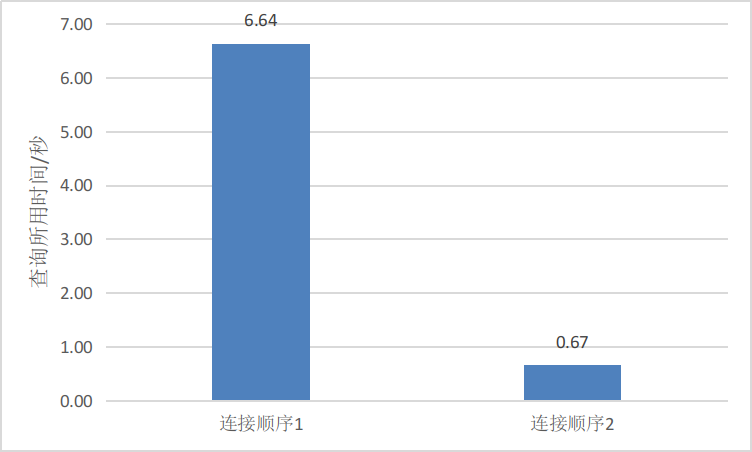
\includegraphics[width = 1\textwidth]{SequenceTime}
    \caption{不同连接顺序所用查询时间}
    \label{SequenceTime}
\end{figure}

\section{马尔可夫决策过程定义和特征化}[MDP]
为了能够把一个优化问题表述为一个强化学习问题,我们需要把问题形式化为一个马尔可夫决策过程(MDP)。而在第二章预备知识中,我们介绍过,一个马尔可夫决策过程可以形式化的表示为五元组\ref{MDP5},所以在本小节中,我们将依次介绍每一个元素在此优化方法中的具体定义,举出相应的例子,之后再根据定义给出其相应的编码方式以便于计算机的识别和处理,即对每个元素进行特征化处理。
\subsection{状态的定义和特征化}[state]
\subsubsection{状态的定义}[definition]
$S$代表Agent所有可能的状态,对任意时刻$t$的状态$S_t$都满足$S_t \in S$。
在我们的优化问题中,我们用$S_t$来表示在t时刻基本图模式(BGP)的连接状态,$S_0$是初始状态,表示还没有开始做连接。

以查询\ref{sparql1}为例子,这个查询中包括6个三元组模式(Triple):$T_1, T_2, T_3, T_4, T_5, T_6$。

以下过程将展示状态是如何随时间变化的:
\begin{enumerate}
    \item 初始时的状态$S_0=\phi$,表示所有的三元组模式都没有连接。
    \item 如果在$t_1$时刻,已经得到了三元组模式$T_1$的查询中间结果,则此时的状态可以表示为$S_{t1} = T_1$; 
    \item 如果在$t_2$时刻,三元组模式$T_1$的查询中间结果与$T_3$的查询中间结果进行了连接操作,则此时的状态可以表示为$S_{t2} = T_1 \Join T_3$;
    \item 如果在$t_3$时刻,前面的连接中间结果又与三元组模式$T_2$的查询中间结果进行了连接操作,则此时的状态可以表示为$S_{t3} = T_1 \Join T_3 \Join T_2$;
    \item 以此类推,如果最终查询结束时,这6个三元组模式(Triple)查询中间结果的连接顺序是$T_1 \Join T_3 \Join T_2 \Join T_5 \Join T_4 \Join T_6$,则在查询处理结束的时刻$t_6$时,状态的表示为$S_{t6} = T_1 \Join T_3 \Join T_2 \Join T_5 \Join T_4 \Join T_6$。
\end{enumerate}

\subsubsection{特征化}[Featurization]
在将以上描述的状态定义进行特征化时,我们面临着两个挑战:
\begin{enumerate}
    \item 如何将一个三元组模式表示为一个编码,如何通过编码来体现这些三元组模式中间查询结果的连接顺序;
    \item 每一个SPARQL查询都有不同的基本图模式(BGP),即如果有两个不同的SPARQL查询,则它们的三元组模式和总个数都不尽相同。而对于强化学习算法来说,其输入数据(状态的特征编码)的维度需要维持衡定,所以如何将个数变化的三元组模式集特征化为一个长度固定的编码是比较困难的。
\end{enumerate}

为了能够解决上面的两个问题,我们需要先介绍三元组模式的两个种类:
\begin{enumerate}
    \item 类型三元组模式(Type triple)。这种三元组的特征是其属性固定为Type的URI: <http://www.w3.org/1999/02/22-rdf-syntax-ns\#type>。类型三元组模式是用来描述三元组$(s,p,o)$中主体($s$)的类型是客体($o$)的一类三元组模式,其形式化表述为:$$Type\ triple \in \lbrace (RDF-T \cup V)\times RDF-Type\times (RDF-T \cup V) ) \rbrace$$ 其中$V$表示变量,$RDF-Type$代表type的URI:<http://www.w3.org/1999/02/22-rdf-syntax-ns\#type>。
    \item 属性三元组模式(Property triple)。这种三元组是所有三元组模式中除去类型三元组后的部分。其用于表示一个三元组$(s,p,o)$中主体($s$)的某属性($p$)是客体($o$)。其形式化表述为:$$Property\ triple \in \lbrace Triple \rbrace - \lbrace Type\ triple \rbrace $$ 其中$\lbrace Triple \rbrace$表示三元组模式的集合,$\lbrace Type\ triple \rbrace$表示类型三元组模式的集合。
\end{enumerate}

例如,三元组模式$T_1$:" ?X rdf:type ub:GraduateStudent " 是一个类型三元组模式,它的查询语义是查询所有类型是研究生(Graduate)的主体(subject)。三元组模式$T_2$:" ?X ub:memberOf ?Z "是一个属性三元组模式,它的查询语义是查询所有符合主体(subject)是客体(object)的成员(member)的三元组。

根据以上的定义,我们首先对输入的SPARQL查询中的三元组模式进行映射。映射规则如下所示:
\begin{equation}
    \label{mapT}
    T_i \rightarrow o, T_i \in \lbrace Type\ triple\rbrace \& T_i = (s,rdf:type,o)   
\end{equation}
\begin{equation}
    \label{mapP}
    T_i \rightarrow p, T_i \in \lbrace Property\ triple\rbrace \& T_i = (s,p,o)   
\end{equation}
对于一个三元组模式,如果它是一个类型三元组模式,则将其映射为它的客体(subject);如果它是一个属性三元组模式,则将其映射为它的属性(property)。这样做映射是因为对于一个属性三元组模式来说,它的客体(subject)最能够反映这个三元组模式的特征,是一个三元组模式最重要的信息,所以用客体来唯一代表三元组模式是合适的。同理,对于属性三元组模式来说,属性(property)是最能反映一个属性三元组模式的信息,所以我们用属性来做属性三元组模式的第一次映射结果。除此之外,在Jena图数据库中,一个类型三元组数据昰以类型值(客体)作为索引项的,一个属性三元组数据昰以属性作为索引项的,所以这样做映射还可以把图数据库的索引也加入到特征中,使得算法的输入数据具有更多的信息。

例如,三元组模式$T_1$:" ?X rdf:type ub:GraduateStudent " 是一个类型三元组模式,根据映射规则\ref{mapT},将其映射为ub:GraduateStudent。三元组模式$T_2$:" ?X ub:memberOf ?Z "是一个属性三元组模式,根据映射规则\ref{mapP},所以将其映射为ub:memberOf。

在获得映射的结果后,我们将每一个映射结果都作为一个单独的特征位,用一个二进制位来表示,0表示该三元组模式的中间查询结果还未被连接,1表示该三元组模式的中间查询结果已经被连接。但是这样还是无法解决不同的基本图模式在特征化后得到的向量维度不统一问题。为了解决这个问题,我们需要在查询优化系统初始化时,就确定好特征化结果的向量维度,将所有查询中可能出现的三元组模式映射结果都罗列出来,形成一个三元组模式映射结果全集M,然后将它们特征化为一个one-hot向量,这个向量的长度是全集M的大小。这样在之后的查询中,每个查询的三元组模式都会是初始时的三元组模式全集M的子集,这样每个查询的特征化结果就都可以变成一个定长向量了。

我们为了在系统初始化时刻获取三元组模式映射结果全集M,需要在系统导入RDF数据时,对导入的数据进行统计。对导入的每一条RDF数据按照映射规则\ref{mapP}和\ref{mapT}进行映射处理,然后收集所有的映射结果形成全集M。算法伪代码见算法\ref{statistics}。
\begin{algorithm}[ht]
    \caption{统计三元组模式映射结果算法}
    \label{statistics}    
    \KwIn{RDF三元组 T} 
    \KwOut{类型三元组模式映射结果全集MT,属性三元组模式映射结果全集MP} 
    初始化类型三元组映射结果集合MT=$\phi $\;
    初始化属性三元组映射结果集合MP=$\phi $\;
    \For{triple$(s_i,p_i,o_i)$ in T}  
    {
        \If{triple是类型三元组 and $o_i$不在集合MT中}
        {
            将$o_i$加入到集合MT中\;
        }
        \ElseIf{triple是属性三元组 and $p_i$不在集合MP中}
        {
            将$p_i$加入到集合MP中\;
        }
    }
\end{algorithm} 

\begin{table}[htbp]
    \caption[table1]{RDF数据}
    \label{RDF2}
    \vspace{0.5em}\centering\wuhao
    \begin{tabular}{|c|c|}
    \toprule[1.5pt]
    RDF三元组& 类型\\
    \midrule[1pt]    
    <student1,rdf:type,GraduateStudent>&类型三元组\\
    <university0,rdf:type,University>&类型三元组\\
    <student1,takesCourse,course1>&属性三元组\\
    <student1,memberOf,department>&属性三元组\\
    <course1,rdf:type,Course>&类型三元组\\
    <department1,rdf:type,Department>&类型三元组\\
    <department1,subOrganizationOf,university0>&属性三元组\\
    \bottomrule[1.5pt]
    \end{tabular}
\end{table}

例如,在系统开始时导入了如表格\ref{RDF2}所示的RDF数据,则在导入时,进行如下统计操作:初始时,集合MT和MP都是空的,在导入三元组<student1,rdf:type,GraduateStudent>时,由于它是类型三元组,根据映射规则\ref{mapT},将GraduateStudent加入到集合MT中;三元组<university0,rdf:type,University>是类型三元组,则将University加入到集合MT中;三元组<student1,takesCourse,course1>是属性三元组,根据映射规则\ref{mapP},将takeCourse加入到集合MP中;三元组<student1,memberOf,department>是属性三元组,则将memberOf加入到集合MP中;三元组<course1,rdf:type,Course>是类型三元组,则将Course加入到集合MT中;三元组<department1,rdf:type,Department>是类型三元组,则将Department加入到集合MT中;三元组<department1,subOrganizationOf,university0>是属性三元组,则将subOrganizationOf加入到集合MP中。

在获得三元组映射结果全集后,将集合中的元素做如下特征化:
\begin{table}[htbp]    
    \vspace{0.5em}\centering\wuhao
    \begin{tabular}{ccccccc}
    \toprule[1.5pt]
    GraduateStudent& University&Course&Department&takesCourse&memberOf&subOrganizationOf\\
    \midrule[1pt]    
    0&0&0&0&0&0&0\\
    \bottomrule[1.5pt]
    \end{tabular}
\end{table}

因为向量中所有二进制位都是0,所以此时以上编码状态处于初始状态$S_0$。
对于在$t_3$时刻,状态为$S_{t3} = T_1 \Join T_3 \Join T_2$,即三元组模式$T_1,T_2,T_3$的中间查询结果已经被连接,这三个三元组模式的映射结果GraduateStudent,memberOf,Department对应的特征位将被设置为1,其特征向量如下:
\begin{table}[htbp]    
    \vspace{0.5em}\centering\wuhao
    \begin{tabular}{ccccccc}
    \toprule[1.5pt]
    GraduateStudent& University&Course&Department&takesCourse&memberOf&subOrganizationOf\\
    \midrule[1pt]    
    1&0&0&1&0&1&0\\
    \bottomrule[1.5pt]
    \end{tabular}
\end{table}

\subsection{动作的定义和特征化}[action]
$A$表示有限动作集(动作空间),对任意时刻$t$的动作$A_t$,都满足$A_t \in A$。
在我们的优化问题中,在某个连接状态下,所有可能的连接动作构成了有限动作集。在t时刻,其连接状态为$S_t$,则此时,所有可能的连接动作就是整个动作空间$A$,而学习者会从动作集中选择一个动作$A_i$去实际执行。动作以选择连接的三元组模式中间结果的编号作为编码。

再以查询\ref{sparql1}为例子,这个查询中包括6个三元组模式(Triple):$T_1, T_2, T_3, T_4, T_5, T_6$。

以下过程将展示动作集和动作是如何随时间变化的:
\begin{enumerate}
    \item 初始时的状态$S_0=\phi$,表示所有的三元组模式都没有连接,此时,可以从剩余的6个三元组模式中任选一个开始执行实际查询,与剩余的6个三元组模式进行连接操作构成了动作集,动作集大小为6,假设学习者选择首先执行三元组模式$T_1$得到其中间查询结果,则它选择的动作是与三元组模式$T_1$的中间查询结果做连接操作,这个动作的编码是三元组模式$T_1$的编号1。
    \item 如果在$t_1$时刻的状态是$S_{t1} = T_1$,此时,可以从剩余的5个三元组模式中间结果$T_2,T_3,T_4,T_5,T_6$中任选一个进行连接操作,动作集大小为5,假设学习者选择与$T_3$的查询中间结果进行连接操作,这个动作的编码就是三元组模式$T_3$的编号3。
    \item 如果在$t_2$时刻,连接状态为$S_{t2} = T_1 \Join T_3$,此时,可以从剩余的4个三元组模式中间结果$T_2,T_4,T_5,T_6$中任选一个进行连接操作,动作集大小为4,假设学习者选择与$T_2$的查询中间结果进行连接操作,这个动作的编码就是三元组模式$T_2$的编号2。
    \item 如果在$t_3$时刻,连接状态为$S_{t3} = T_1 \Join T_3 \Join T_2$,此时,可以从剩余的3个三元组模式中间结果$T_4,T_5,T_6$中任选一个进行连接操作,动作集大小为3,假设学习者选择与$T_5$的查询中间结果进行连接操作,这个动作的编码就是三元组模式$T_5$的编号5。
    \item 以此类推,在每个状态下,选择从动作集中选择一个动作执行,直到最后的状态是所有的三元组模式的中间结果都得到连接,即得到了最终的查询结果为止。
\end{enumerate}
状态转换的规则是在一个状态$S_t$下,如果学习者选择了动作$a_i$,则将状态$S_t$的编码中三元组模式$T_i$对应的特征位置1,状态由$S_t$转换成了状态$S_{t+1}$。
\subsection{奖励定义}[reward]
奖励(reward)是学习者执行一个动作后环境给予的回馈信息,用于告知学习者这个动作执行的结果,来帮助学习者学习这个动作带来的价值。在我们的查询优化问题中,在查询优化器生成一个查询计划后,交给了底层RDF存储去执行查询计划,查询优化器将通过执行来学习该查询计划的好坏,一个查询计划执行的代价越小,说明该查询计划的效率越高,越应该获得更高的奖励值。

我们首先想到将查询计划执行时间t的负数作为奖励值,因为查询时间t越小,说明查询的效率越高,这样学习者获得的奖励-t就越大。但是这样的话还存在两个问题:
\begin{enumerate}
    \item 在实际的执行过程中,查询计划的执行时间变化幅度很大,其范围在100到$10^6$之间,而深度强化学习方法通常能够处理的奖励值范围是-10到10之间,幅度过大的奖励值对模型的训练会造成极大的干扰。
    \item 在实际训练模型时,由于连接顺序的可能情况很多,模型不可能探索所有可能的连接顺序,对于没有被强化学习探索过的连接顺序,由于查询计划没有被实际被执行过,所以对应的奖励值是0。而所有已经被探索过的连接顺序的奖励值都是小于0的,这样就造成模型会认为奖励值为0的连接顺序更优,模型最终总会把没有被探索过的连接顺序作为最优解,模型无法正常的运作。
\end{enumerate}

为了解决第一个问题,我们可以通过对奖励进行归一化,来避免奖励值出现较大的变化幅度,而对于第二个问题,我们可以通过对奖励值进行一些变换使得所有的奖励值都是大于0,并且能够满足奖励值随着查询代价的减小而增大。综上两个目的和方法,我们将奖励值定义如下:
\begin{equation}
    R(S=s_t,A=a_i)=e^{-t}*10
\end{equation}
其中t是查询计划的执行时间。通过以上定义,我们将奖励值的范围限定为0到10之间,来满足深度强化学习常用的奖励数值范围。如图\ref{reward}展现了奖励值随查询时间的变化关系,随着查询时间的变长,奖励值会逐渐趋向于0,查询时间越接近0,奖励值就越接近最大值10,这样的对应关系就可以解决上文提到的两个问题。
\begin{figure}[h]
    \centering
    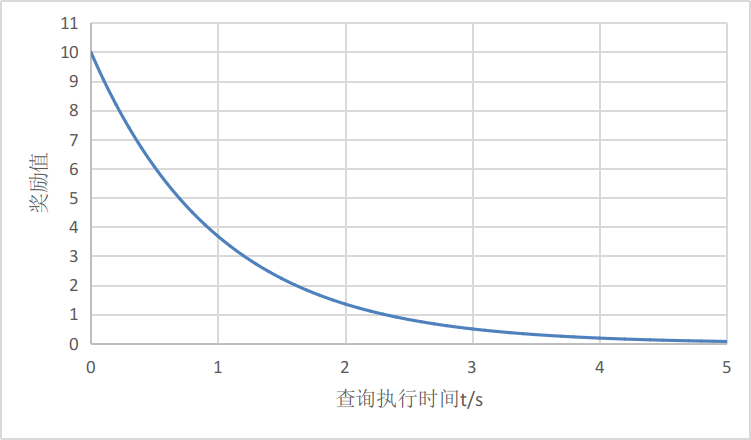
\includegraphics[width = 1\textwidth]{reward}
    \caption{奖励值随查询时间的变化}
    \label{reward}
\end{figure}
\section{本章小结}
在这一章节中,我们提出了一种基于强化学习的方法来对SPARQL查询中基本图模式查询进行优化,该方法能够优化基本图模式中的三元组模式中间查询结果的连接顺序,从而到达提高查询效率的目的。我们首先对SPARQL的基本图模式优化问题进行了详细的描述,展现了其较大的优化空间,确定了该优化问题的输出输出。之后,我们从马尔可夫决策过程的五元组(状态,动作,策略,奖励,初始状态)开始,分别详细得介绍了状态、初始状态、动作的定义和特征化方法,然后通过举例的方式描述了状态之间的转换方式,最后介绍了奖励值的计算方法。

\chapter{强化学习算法的实现和实验结果}
在这章中,首先我们将基于Apache Jena开源图数据库,介绍基于强化学习的SPARQL优化方法的具体实现,然后介绍搭建的实验环境的参数,最后,我们使用标准测试数据(Benchmark)来验证方法的有效性并进行不同算法之间的效果比较。
\section{强化学习算法的实现}
我们的算法基于Q学习算法和深度Q学习算法,但是我们根据实际的问题情景,对两个算法进行了一些改进,以达到更高的效率和准确度。以下内容我们将对使用的框架和算法的改进部分进行介绍。
\subsection{Q学习算法实现}
在第二章中,我们已经介绍过基本的Q学习算法,在这里我们将描述我们对数据结构的特殊设计。

Q 学习算法需要一个Q值表来存储(状态,动作)与Q值的映射,但是考虑到基本图模式连接状态的空间复杂度是$n!$,动作最多有n个,则如果使用二维矩阵来存储Q值需要$n*n!$的存储空间,n是三元组模式映射结果全集M的大小,这样的存储方式需要的空间极大,在n值为13时就需要大约60Gb内存,同时内存利用率也极低。因为连接状态空间极大,强化学习模型经过大量训练也只能探索极小的一部分空间,所以Q值表其实是一个稀疏矩阵。为了提高空间利用率,我们可以用HashMap来存储(状态,动作)与Q值的映射。我们用于存储Q值表的数据结构为Map<List<String>, Map<String, Double>>,其中:
\begin{itemize}
    \item List<String>用于存储连接状态。String存储的是三元组模式根据映射规则\ref{mapT}和\ref{mapP}得到的结果,List<String>中元素的顺序代表当前状态下三元组模式中间结果的连接顺序。
    \item Map<String,Double>用于存储动作和Q值的映射。String存储的也是三元组模式的映射结果,但是它代表在当前状态下选择连接的三元组模式,是代表的连接动作,Double类型用于存储Q值,Map数据结果用于存储动作选择和Q值的映射关系。
    \item Map<List,Map>用于存储状态与动作的映射关系。
\end{itemize}

\subsection{深度Q学习算法(DQN)}
由于我们选用的图数据库是Apache Jena,它是使用Java语言实现的,所以我们在实现深度Q学习算法时,为了方便与数据库进行交互,选择了一个由Java语言实现的强化学习库RL4J(Reinforcement Learning for java),它的神经网络部分是由DeepLearning4J来完成的。我们对RL4J中的MDP类(负责马尔可夫决策过程)进行了重写,将状态,动作,状态转换,奖励和初始化操作根据章节三的方法进行了实现。特别的是,由于我们的动作定义的特殊性,我们需要对框架中的动作空间部分进行定制。与框架中的实现不同的是,我们的方法在每次状态更新后,合法的动作都会减少1个,动作空间需要更新,然后学习者再从更新的动作空间中选择一个动作去执行。

\section{实验环境}
本文的实验是在一台笔记本电脑上进行的,该电脑的CPU是双核Intel Core i7 6500U(2.5 GHz - 3.10 GHz),8GB内存;显卡是Nvidia GeForce 940MX(1122 MHz - 1242 MHz),显存2GB,显卡驱动版本是440.82,CUDA版本是10.2;电脑运行的系统是Ubuntu 18.04。

我们使用的Java是OpenJDK1.8.0,使用的Apache Jena版本是3.14.0,使用的RDF底层存储是TDB。我们使用的标准测试数据是LUBM\cite{LUBM},这个基准测试是由Lehigh大学发起,旨在以一种标准且系统的方式进行语义Web存储库的评估工作。LUBM由大学领域的本体组成,可自定义和可重复的合成数据,包括14个标准SPARQL查询。
\section{实验结果}
\section{本章小结}
在本章中,我们首先介绍了强化学习算法的实现,包括Q学习算法和深度Q学习算法的实现,特别介绍了我们根据实际问题情景对算法的改进部分。之后介绍了实验的环境,包括CPU、GPU、操作系统和基准测试。最后,我们给出了实验中两种算法的实测结果,通过与随机连接顺序的查询效率和Jena自带优化器查询效率进行比较,来验证本文优化方法的有效性。
% Local Variables:
% TeX-master: "../main"
% TeX-engine: xetex
% End:
